\documentclass[12pt,a4paper]{article}
\usepackage[utf8]{inputenc}
\usepackage[T1]{fontenc}
\usepackage{amsmath,amssymb,amsfonts}
\usepackage{graphicx}
\usepackage{booktabs}
\usepackage{longtable}
\usepackage{hyperref}
\usepackage{listings}
\usepackage{xcolor}
\usepackage{algorithm}
\usepackage{algpseudocode}
\usepackage{tikz}
\usetikzlibrary{shapes,arrows,positioning,fit}
\usepackage{float}
\usepackage{subcaption}
\usepackage{geometry}
\geometry{margin=1in}
\usepackage{setspace}
\onehalfspacing

% Code listing style
\lstset{
    basicstyle=\ttfamily\small,
    breaklines=true,
    frame=single,
    numbers=left,
    numberstyle=\tiny\color{gray},
    keywordstyle=\color{blue},
    commentstyle=\color{green!60!black},
    stringstyle=\color{red},
    backgroundcolor=\color{gray!10}
}

\title{\textbf{Automated Incident Response Using Deep Reinforcement Learning}\\
\large A Comprehensive Technical Report}
\author{Pratyush Kumar}
\date{January 2026}

\begin{document}

\maketitle

\begin{abstract}
This report presents a comprehensive study on the application of Deep Reinforcement Learning (DRL) for automated incident response in cybersecurity systems. We develop a custom Gymnasium environment that simulates realistic attack scenarios including brute force and ransomware attacks, using parameters extracted from the CICIDS 2017 and CERT Insider Threat datasets. Our Deep Q-Network (DQN) agent, employing Dueling architecture and Double DQN techniques, learns to make optimal defensive decisions by interacting with this simulated environment. Through extensive experimentation, we demonstrate that our DRL-based approach significantly outperforms traditional rule-based systems including Snort-inspired, NIST 800-61, and MITRE ATT\&CK pattern matching baselines. Statistical significance testing using independent samples t-tests, Cohen's d effect sizes, and 95\% confidence intervals validates our findings. The agent achieves a 75\% success rate with statistically significant improvements over all baseline approaches (p < 0.05), including a Cohen's d of 4.32 against the random baseline and 0.30 against the threshold-based approach.
\end{abstract}

\tableofcontents
\newpage

%==============================================================================
\section{Introduction}
%==============================================================================

\subsection{Background and Motivation}

The cybersecurity landscape has evolved dramatically over the past decade, with organizations facing an unprecedented volume and sophistication of cyber threats. Traditional security measures, while still essential, struggle to keep pace with the rapidly evolving tactics employed by malicious actors. Security Information and Event Management (SIEM) systems and Intrusion Detection Systems (IDS) represent the cornerstone of enterprise security monitoring, yet their reliance on predefined rules and signatures creates fundamental limitations in detecting novel attack patterns and responding to threats in real-time.

The challenge of incident response extends beyond mere detection. Security analysts face an overwhelming volume of alerts, many of which are false positives, while simultaneously needing to make rapid decisions about appropriate defensive actions. The cognitive load on human analysts, combined with the speed at which modern attacks propagate, creates a compelling case for intelligent automation in incident response. Machine learning approaches have shown promise in various security applications, from malware classification to network anomaly detection. However, the sequential decision-making nature of incident response—where actions taken influence future states and outcomes—makes this domain particularly well-suited for reinforcement learning approaches.

This research explores the application of Deep Reinforcement Learning to create an adaptive, intelligent incident response system capable of learning optimal defensive strategies through interaction with a simulated environment. By framing incident response as a Markov Decision Process, we enable an agent to learn complex temporal dependencies and develop nuanced response strategies that account for the evolving nature of attacks.

\subsection{Problem Statement}

The core challenge addressed in this work is the development of an autonomous agent capable of making effective incident response decisions given only observable system metrics. Specifically, given a continuous stream of system observables including login attempt rates, file access patterns, and CPU utilization, the agent must learn to detect ongoing attacks from inherently noisy observations, select appropriate defensive actions from a discrete action space to contain threats effectively, minimize false positive responses that could disrupt legitimate operations, and generalize learned policies across different attack types and scenarios without explicit programming of detection rules.

The problem is inherently challenging due to several factors. First, the observations available to the agent are noisy approximations of the true system state, mirroring the uncertainty faced by real security systems. Second, the consequences of actions are not immediately apparent—a premature response may constitute a false positive, while delayed action may allow an attack to progress. Third, the optimal policy must balance the tradeoff between aggressive defense (risking disruption) and conservative monitoring (risking compromise).

\subsection{Contributions}

This work makes several significant contributions to the intersection of reinforcement learning and cybersecurity. We design and implement a custom Gymnasium environment that faithfully simulates realistic incident response scenarios, complete with probabilistic attack progression and stochastic defender action outcomes. The environment incorporates a 10-dimensional enhanced observation space that includes not only raw metrics but also rate-of-change features and moving averages to facilitate attack detection.

We develop attack simulators based on Finite State Machines with parameters derived from real-world datasets, specifically the CICIDS 2017 network intrusion dataset and the CERT Insider Threat dataset. These simulators model the progressive nature of actual attacks, from initial reconnaissance through exploitation to system compromise.

Our implementation of Deep Q-Networks incorporates both Double DQN to reduce overestimation bias and Dueling architecture to separate state value estimation from action advantage computation. This combination provides stable training and improved generalization across states where action choice matters differentially.

We provide comprehensive baseline comparisons against implementations inspired by established security frameworks including Snort IDS threshold-based detection, NIST SP 800-61 incident handling guidelines, and MITRE ATT\&CK technique pattern matching. These baselines, while simplified representations of their respective frameworks, capture the essential decision-making logic and provide meaningful points of comparison.

Finally, we conduct rigorous statistical validation of our results using independent samples t-tests, Cohen's d effect sizes, and 95\% confidence intervals. This analysis provides strong evidence for the effectiveness of our approach and quantifies the magnitude of improvement over baseline methods.

\subsection{Report Organization}

The remainder of this report is organized as follows. Section 2 reviews related work in intrusion detection, machine learning for cybersecurity, and reinforcement learning applications in security domains. Section 3 describes our methodology in detail, including the environment design, attack simulation, DQN architecture, and training process. Section 4 presents experimental results and comprehensive statistical analysis. Section 5 discusses our findings, limitations, and practical implications. Section 6 concludes with a summary and directions for future work.

%==============================================================================
\section{Related Work}
%==============================================================================

\subsection{Intrusion Detection Systems}

The field of intrusion detection has a rich history spanning several decades, with systems traditionally categorized into signature-based and anomaly-based approaches. Signature-based systems, exemplified by Snort, maintain databases of known attack patterns and match observed traffic or behavior against these signatures. While highly effective for detecting known threats with low false positive rates, these systems are fundamentally reactive—they cannot detect attacks for which no signature exists. The constant need for signature updates and the inability to detect zero-day exploits represent significant limitations in modern threat environments.

Anomaly-based detection systems take a complementary approach by establishing baselines of normal behavior and flagging deviations from these baselines as potentially malicious. These systems offer the theoretical advantage of detecting novel attacks without requiring prior knowledge of their signatures. However, they face practical challenges including high false positive rates due to legitimate behavioral variations, difficulty in defining "normal" in dynamic environments, and susceptibility to evasion through gradual behavioral modification. The balance between sensitivity (catching attacks) and specificity (avoiding false alarms) remains a central challenge in anomaly detection research.

\subsection{Machine Learning in Cybersecurity}

The application of machine learning to cybersecurity problems has grown substantially in recent years, driven by both increased data availability and advances in learning algorithms. Random Forests and Support Vector Machines have been successfully applied to network intrusion detection, leveraging feature engineering from packet headers and flow statistics. Deep Neural Networks have demonstrated remarkable capability in malware classification tasks, learning hierarchical representations directly from raw binary or behavioral features.

Autoencoders have proven particularly valuable for anomaly detection, learning compressed representations of normal behavior and using reconstruction error as an anomaly score. This unsupervised approach addresses the challenge of obtaining labeled attack data for training. Recurrent Neural Networks, including Long Short-Term Memory (LSTM) networks, have been applied to sequence-based attack detection, capturing temporal dependencies in network traffic or system call sequences that may indicate multi-stage attacks.

Despite these advances, most machine learning approaches to security are supervised or unsupervised learning methods that classify individual observations or sequences. They do not inherently address the sequential decision-making problem of incident response—determining what action to take in response to detected threats and how to balance multiple objectives over time.

\subsection{Reinforcement Learning for Security}

Reinforcement learning offers a natural framework for sequential decision-making under uncertainty, making it well-suited for security applications where actions have consequences that unfold over time. Researchers have applied RL to autonomous penetration testing, training agents to discover vulnerabilities in simulated networks. Others have explored adaptive honeypot configuration, where agents learn to present deceptive services that maximize attacker engagement and intelligence gathering.

Network defense games represent another active area, modeling the interaction between attackers and defenders as a game-theoretic problem where RL agents learn defensive strategies. Automated vulnerability assessment systems have used RL to prioritize security testing efforts based on learned patterns of vulnerability occurrence.

Our work differs from prior RL security research by focusing specifically on the incident response decision-making process—the challenge of selecting appropriate defensive actions given uncertain observations of potentially malicious activity. We emphasize the use of realistic attack simulations grounded in empirical data and provide rigorous comparison against established security frameworks.

\subsection{Security Frameworks and Standards}

Our baseline comparisons draw from three established security resources. Snort is an open-source network intrusion prevention system that combines signature matching, protocol analysis, and anomaly detection. Its rule-based approach exemplifies traditional IDS design philosophy. NIST Special Publication 800-61, the Computer Security Incident Handling Guide, provides comprehensive guidance on establishing incident response capabilities and categorizing incidents by functional impact. The MITRE ATT\&CK framework has become an essential resource for understanding adversary tactics and techniques, organizing known attack patterns into a structured knowledge base that supports detection and response planning.

%==============================================================================
\section{Methodology}
%==============================================================================

\subsection{System Architecture}

Our system follows the standard reinforcement learning paradigm of an agent interacting with an environment through a cycle of observation, action, and reward. The environment encapsulates the attack simulation and observation generation, presenting the agent with a 10-dimensional state vector at each timestep. The agent, implemented as a Dueling Double DQN, processes this observation through a neural network to estimate action values and selects actions according to an epsilon-greedy policy. The environment responds to each action by potentially containing an ongoing attack, generating a reward signal, and producing the next observation.

The modular design separates concerns cleanly: the attack simulator manages attack state transitions and observable metric generation; the environment wrapper implements the Gymnasium interface and handles reward calculation; and the agent encapsulates the neural network architecture, experience replay, and learning algorithm. This separation facilitates experimentation with different attack types, reward structures, and learning algorithms.

\begin{figure}[H]
\centering
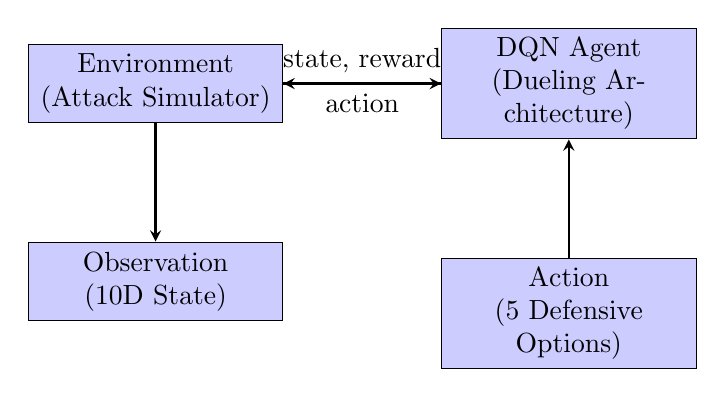
\begin{tikzpicture}[
    node distance=1.5cm,
    block/.style={rectangle, draw, fill=blue!20, text width=3cm, text centered, minimum height=1cm},
    arrow/.style={thick,->,>=stealth}
]
    \node[block] (env) {Environment\\(Attack Simulator)};
    \node[block, right=2cm of env] (agent) {DQN Agent\\(Dueling Architecture)};
    \node[block, below=of env] (obs) {Observation\\(10D State)};
    \node[block, below=of agent] (action) {Action\\(5 Defensive Options)};
    
    \draw[arrow] (env) -- node[above] {state, reward} (agent);
    \draw[arrow] (agent) -- node[below] {action} (env);
    \draw[arrow] (env) -- (obs);
    \draw[arrow] (action) -- (agent);
\end{tikzpicture}
\caption{High-level system architecture showing the interaction between the DQN agent and the incident response environment.}
\label{fig:architecture}
\end{figure}

\subsection{Custom Gymnasium Environment}

Our environment implements the standard Gymnasium API, ensuring compatibility with established RL libraries and facilitating reproducibility. The observation space is defined as a continuous 10-dimensional box, while the action space consists of five discrete defensive options. Each episode runs for a maximum of 100 timesteps, representing a monitoring window during which zero or more attacks may occur and the agent must respond appropriately.

The observation space design reflects careful consideration of what information would realistically be available to an automated security system. Raw metrics—login attempt rate, file access rate, and CPU utilization—provide the foundation. To these, we add derived features that enhance the agent's ability to detect attacks. Rate-of-change values for each metric capture sudden spikes characteristic of attack onset. Moving averages computed over a 10-step window smooth noise and highlight sustained anomalies. A sustained anomaly indicator tracks how long metrics have remained elevated, helping distinguish brief legitimate spikes from persistent attack activity. Finally, a normalized time feature indicates progress through the episode.

The action space provides the agent with five response options of increasing severity. The do\_nothing action represents continued monitoring without intervention, appropriate when observations fall within normal ranges. Block\_ip instructs the system to block network traffic from a suspicious source address. Lock\_account freezes a potentially compromised user account. Terminate\_process kills suspicious executing processes. Isolate\_host represents the most aggressive response, quarantining an entire machine from the network. Each action carries different costs and effectiveness depending on the attack type and stage.

\subsection{Attack Simulator Design}

Attacks are modeled as Finite State Machines (FSMs) with probabilistic transitions between states. This design reflects the reality that attacks typically progress through distinct phases—from initial reconnaissance through active exploitation to eventual compromise—and that defensive actions can interrupt this progression with probability depending on the attack stage and action taken.

The brute force attack simulator models SSH credential stuffing attacks. In the idle state, the system operates normally with baseline metrics. With probability 0.15 per timestep, an attack initiates and transitions to the probing state, representing reconnaissance activity. Observable metrics increase moderately as the attacker probes for vulnerable accounts. With probability 0.2 per timestep in probing, the attack escalates to the active state, characterized by intensive login attempts. Finally, with probability 0.15 from the active state, the attack succeeds and transitions to compromised, representing a successful account breach. The compromised state is terminal, ending the episode with maximum penalty.

The ransomware attack simulator models file encryption attacks through four states. The execution state represents initial malware execution, characterized by elevated CPU usage as malicious code runs. The encryption state shows dramatic increases in file access rates as the ransomware encrypts user files. The data\_loss state represents successful completion of encryption with ransom note deployment. Transition probabilities and observable metrics were calibrated using patterns from the CICIDS 2017 and CERT datasets, ensuring realistic attack signatures.

\begin{figure}[H]
\centering
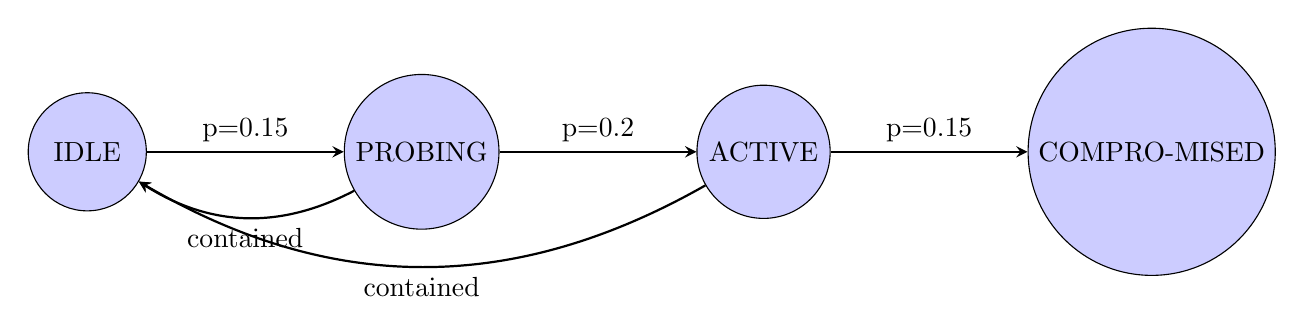
\begin{tikzpicture}[
    node distance=2.5cm,
    state/.style={circle, draw, fill=blue!20, minimum size=1.5cm},
    arrow/.style={thick,->,>=stealth}
]
    \node[state] (idle) {IDLE};
    \node[state, right=of idle] (probe) {PROBING};
    \node[state, right=of probe] (active) {ACTIVE};
    \node[state, right=of active] (comp) {COMPRO-\\MISED};
    
    \draw[arrow] (idle) -- node[above] {p=0.15} (probe);
    \draw[arrow] (probe) -- node[above] {p=0.2} (active);
    \draw[arrow] (active) -- node[above] {p=0.15} (comp);
    
    \draw[arrow, bend left=30] (probe) to node[below] {contained} (idle);
    \draw[arrow, bend left=30] (active) to node[below] {contained} (idle);
\end{tikzpicture}
\caption{Brute Force Attack Finite State Machine showing states and transition probabilities.}
\label{fig:bruteforce_fsm}
\end{figure}

Defender actions have probabilistic effectiveness that varies by attack state, reflecting the reality that earlier intervention is generally more effective. For example, blocking an IP address has 90\% effectiveness during probing but only 30\% effectiveness after compromise, when the attacker may have established multiple access vectors. Isolating the host remains effective across all stages but carries higher operational cost. This design creates interesting tradeoffs for the agent to learn—more aggressive actions have higher effectiveness but also higher false positive costs.

\subsection{Reward Function Design}

The reward function encodes our objectives for the incident response agent, balancing attack containment against operational disruption. Early containment of attacks (during stages 0-1) receives the highest reward of +50, strongly incentivizing rapid response to detected threats. Late containment (stage 2+) still receives a positive reward of +20, recognizing that even delayed response has value. Correct inaction during normal operation receives a small positive reward of +1, teaching the agent patience and reducing false positive tendency.

Penalties are designed to discourage undesirable behaviors. False positives—taking defensive action when no attack is occurring—incur a -10 penalty, reflecting the operational cost of unnecessary interventions. Missing an attack that progresses to compromise receives a severe -30 penalty. Redundant actions (taking the same action multiple times) receive a -5 penalty to encourage action diversity. A small -0.1 step penalty creates time pressure, discouraging indefinite waiting.

\subsection{DQN Agent Architecture}

Our agent implements Deep Q-Learning with two important architectural enhancements: Double DQN and Dueling networks. Standard DQN uses the same network both to select and evaluate actions, leading to overestimation of Q-values. Double DQN addresses this by using the online network to select the best action but the target network to evaluate its value, reducing estimation bias and improving stability.

The Dueling architecture separates the Q-value estimation into two streams: a value stream V(s) estimating the value of being in a state, and an advantage stream A(s,a) estimating the relative value of each action. These combine according to the formula Q(s,a) = V(s) + (A(s,a) - mean(A)), with the mean subtraction ensuring identifiability. This factorization allows the network to learn state values even in states where action choice matters little, improving sample efficiency and generalization.

The network architecture consists of shared hidden layers with 128 and 64 units respectively, using ReLU activation. The value stream adds a 32-unit layer followed by a single output. The advantage stream similarly adds a 32-unit layer followed by five outputs (one per action). Training uses Adam optimization with learning rate 0.001, and the target network synchronizes with the online network every 10 episodes.

\begin{figure}[H]
\centering
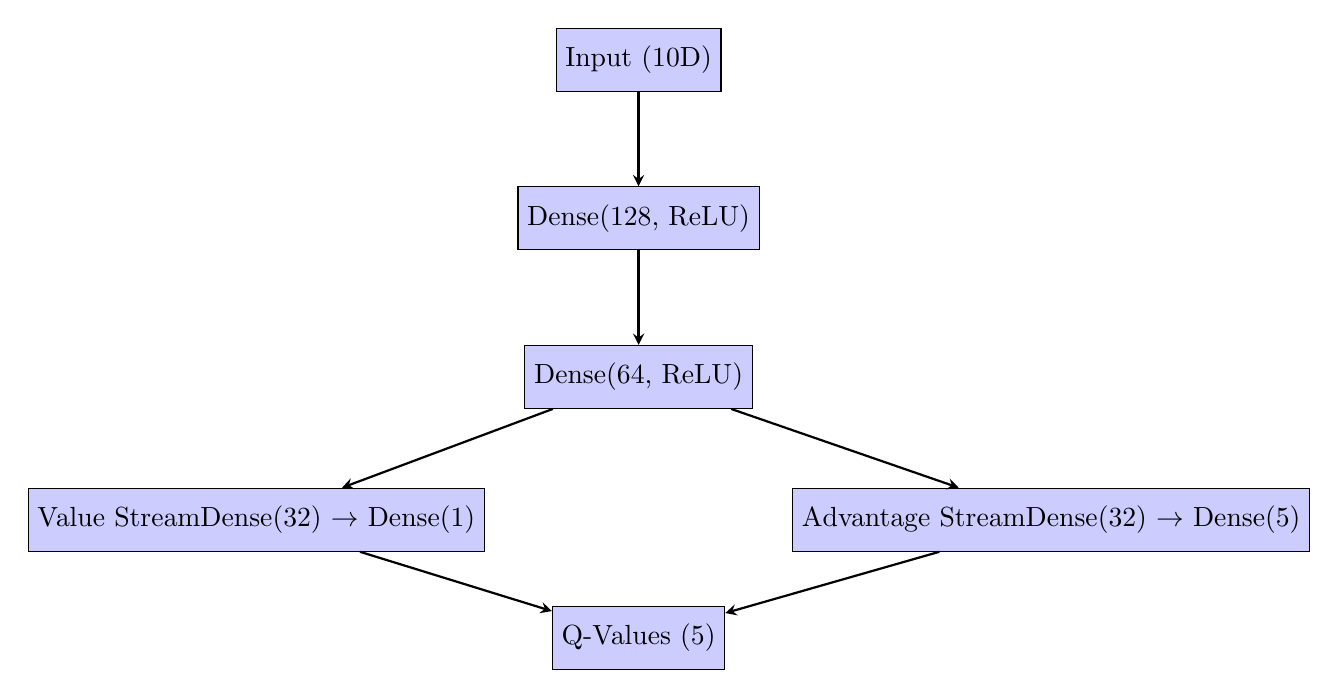
\begin{tikzpicture}[
    node distance=1.2cm,
    layer/.style={rectangle, draw, fill=blue!20, minimum width=2cm, minimum height=0.8cm},
    arrow/.style={thick,->,>=stealth}
]
    \node[layer] (input) {Input (10D)};
    \node[layer, below=of input] (fc1) {Dense(128, ReLU)};
    \node[layer, below=of fc1] (fc2) {Dense(64, ReLU)};
    
    \node[layer, below left=1cm and 0.5cm of fc2] (value) {Value Stream\\Dense(32) $\rightarrow$ Dense(1)};
    \node[layer, below right=1cm and 0.5cm of fc2] (adv) {Advantage Stream\\Dense(32) $\rightarrow$ Dense(5)};
    
    \node[layer, below=2.5cm of fc2] (output) {Q-Values (5)};
    
    \draw[arrow] (input) -- (fc1);
    \draw[arrow] (fc1) -- (fc2);
    \draw[arrow] (fc2) -- (value);
    \draw[arrow] (fc2) -- (adv);
    \draw[arrow] (value) -- (output);
    \draw[arrow] (adv) -- (output);
\end{tikzpicture}
\caption{Dueling DQN Network Architecture showing the separation of value and advantage streams.}
\label{fig:dueling_arch}
\end{figure}

\subsection{Training Process}

Training proceeds through 1000 episodes, with each episode consisting of up to 100 timesteps of environment interaction. The agent follows an epsilon-greedy policy for action selection, with epsilon decaying from 1.0 to 0.01 according to an exponential schedule with decay rate 0.995. This ensures extensive exploration in early training while transitioning to predominantly exploitative behavior as the policy improves.

Each transition is stored in an experience replay buffer with capacity 10,000. Training samples minibatches of 64 transitions uniformly from this buffer, breaking the correlation between consecutive samples that would otherwise destabilize learning. The use of a target network, updated every 10 episodes, provides stable training targets and prevents the moving target problem that plagues online temporal difference learning.

\subsubsection{Training Algorithm}

The complete training procedure is presented in Algorithm \ref{alg:dqn_training}. The algorithm follows the standard DQN training loop with Double DQN target computation and periodic target network updates.

\begin{algorithm}[H]
\caption{DQN Training Loop}
\label{alg:dqn_training}
\begin{algorithmic}[1]
\State Initialize Q-network $Q_\theta$ with random weights
\State Initialize target network $Q_{\theta^-} \leftarrow Q_\theta$
\State Initialize replay buffer $\mathcal{D}$
\For{episode $= 1$ to $N$}
    \State Reset environment: $s_0 \leftarrow$ env.reset()
    \For{step $= 1$ to $T$}
        \State Select action: $a \leftarrow \epsilon\text{-greedy}(Q_\theta(s))$
        \State Execute action: $s', r, done \leftarrow$ env.step($a$)
        \State Store transition: $\mathcal{D} \leftarrow \mathcal{D} \cup \{(s, a, r, s', done)\}$
        \State Sample minibatch from $\mathcal{D}$
        \State Compute targets using Double DQN
        \State Update $Q_\theta$ via gradient descent
        \State $s \leftarrow s'$
        \If{done}
            \State \textbf{break}
        \EndIf
    \EndFor
    \State Decay $\epsilon$
    \If{episode mod 10 $= 0$}
        \State Update target network: $Q_{\theta^-} \leftarrow Q_\theta$
    \EndIf
\EndFor
\end{algorithmic}
\end{algorithm}

\subsubsection{Weight Update Formula}

The Q-network weights are updated using gradient descent on the temporal difference error. For Double DQN, the target Q-value is computed as:

\begin{equation}
y_i = r_i + \gamma \cdot Q_{\theta^-}(s'_i, \arg\max_{a'} Q_\theta(s'_i, a')) \cdot (1 - d_i)
\end{equation}

where $r_i$ is the reward, $\gamma = 0.99$ is the discount factor, $s'_i$ is the next state, and $d_i$ is the terminal flag. The key insight of Double DQN is that the online network $Q_\theta$ selects the best action, while the target network $Q_{\theta^-}$ evaluates its value, reducing overestimation bias.

The loss function is the Huber loss over the minibatch:

\begin{equation}
\mathcal{L}(\theta) = \frac{1}{N} \sum_{i=1}^{N} L_\delta(Q_\theta(s_i, a_i) - y_i)
\end{equation}

The weights are then updated using the Adam optimizer with gradient clipping:

\begin{equation}
\theta \leftarrow \theta - \alpha \cdot \text{Adam}(\nabla_\theta \mathcal{L}(\theta))
\end{equation}

where $\alpha = 0.001$ is the learning rate. Gradients are clipped to have maximum norm 1.0 to prevent exploding gradients.

\subsubsection{Loss Function}

The network is trained using Huber loss (also known as Smooth L1 loss), which combines the benefits of Mean Squared Error for small errors with the robustness of Mean Absolute Error for large errors:

\begin{equation}
L_\delta(a) = \begin{cases} 
\frac{1}{2}a^2 & \text{if } |a| \leq \delta \\
\delta(|a| - \frac{1}{2}\delta) & \text{otherwise}
\end{cases}
\end{equation}

where $\delta = 1.0$ and $a$ is the temporal difference error $Q_\theta(s, a) - y$. This loss function provides stability during training by preventing large gradient updates from outlier experiences.

\subsubsection{Epsilon-Greedy Schedule}

The exploration rate $\epsilon$ decays exponentially according to:

\begin{equation}
\epsilon_t = \max(\epsilon_{end}, \epsilon_{start} \times \epsilon_{decay}^t)
\end{equation}

With $\epsilon_{start} = 1.0$, $\epsilon_{end} = 0.01$, and $\epsilon_{decay} = 0.995$, this produces the following schedule:

\begin{table}[H]
\centering
\caption{Epsilon Decay Schedule}
\begin{tabular}{lcc}
\toprule
\textbf{Episode} & \textbf{Epsilon} & \textbf{Exploration Rate} \\
\midrule
0 & 1.00 & 100\% random \\
100 & 0.61 & 61\% random \\
200 & 0.37 & 37\% random \\
300 & 0.22 & 22\% random \\
500 & 0.08 & 8\% random \\
1000 & 0.01 & 1\% random \\
\bottomrule
\end{tabular}
\end{table}


%==============================================================================
\section{Baseline Agents}
%==============================================================================

\subsection{Random Agent}

The random baseline serves as a lower bound on performance, representing an agent with no learned or programmed knowledge of appropriate responses. At each timestep, it selects uniformly at random from the five available actions. While clearly not a practical approach, this baseline is essential for validating that our learned agent has acquired meaningful behavior—any reasonable approach should significantly outperform random action selection.

\subsection{Threshold Agent}

The threshold-based agent implements simple rule-based detection using fixed thresholds on observable metrics. This approach mirrors basic SIEM alert configurations commonly found in practice. When the login rate exceeds 50 and file rate exceeds 100, the agent selects the most aggressive response of host isolation. When only login rate exceeds 50, account lockout is selected. Moderate login elevation above 30 triggers IP blocking. Elevated file access above 100 triggers process termination. When no thresholds are exceeded, the agent monitors without intervention. Despite its simplicity, this baseline captures the essential logic of many deployed security systems and provides a meaningful comparison point.

\subsection{Snort-Inspired Agent}

This baseline draws inspiration from Snort IDS thresholding rules, implementing detection patterns similar to those used in real network intrusion detection. The agent defines thresholds based on Snort rule conventions—an SSH brute force threshold of 10 login attempts triggers low-level alerting, while exceeding 30 attempts triggers critical response. Rapid file access combined with CPU anomalies triggers ransomware-specific responses. While this implementation uses metric thresholds rather than true packet inspection, it captures the conceptual approach of signature-based IDS systems.

\subsection{NIST 800-61 Agent}

Following the incident response guidelines from NIST Special Publication 800-61, this agent calculates a weighted impact score from observable metrics and selects responses based on impact severity. The scoring weights login and file access impacts at 0.4 each and CPU impact at 0.2, reflecting their relative importance for security assessment. Response selection follows the NIST incident categorization scheme—high impact (score > 0.8) warrants immediate isolation, while lower impact levels receive proportionally less aggressive responses. This baseline represents a principled approach to incident response based on established government guidelines.

\subsection{MITRE ATT\&CK Agent}

The MITRE ATT\&CK baseline attempts to detect specific attack techniques from the ATT\&CK framework based on observable patterns. Elevated login rates trigger detection of technique T1110 (Brute Force), with higher rates escalating to T1110.001 (Password Guessing). Combined file access and CPU anomalies trigger detection of T1486 (Data Encrypted for Impact), corresponding to ransomware activity. Response severity corresponds to the most serious detected technique. While this implementation is simplified compared to full ATT\&CK-based detection, it demonstrates the concept of technique-aware response selection.

%==============================================================================
\section{Experimental Results}
%==============================================================================

\subsection{Training Performance}

Training was conducted for 1000 episodes using the configuration described in Section 3. The learning curve demonstrates clear improvement over the course of training, with the agent progressing from random behavior through exploration to effective defensive policy. Figure \ref{fig:learning_curve} shows the episode rewards over training, with a moving average window highlighting the improvement trend.

\begin{figure}[H]
\centering
\includegraphics[width=0.9\textwidth]{figures/learning_curve.png}
\caption{Learning curve showing episode rewards over 1000 training episodes. The moving average (orange line) demonstrates steady improvement from negative rewards in early training to positive rewards in later episodes.}
\label{fig:learning_curve}
\end{figure}

The training process exhibited the expected pattern of initially poor performance during the high-exploration phase, followed by rapid improvement as the policy learned basic attack detection, and finally convergence to stable performance. In the first 100 episodes, the agent achieved mean reward of approximately -200 while epsilon remained high, indicating extensive random exploration. By episodes 301-500, mean reward improved to approximately +15 as the agent learned to recognize attacks and take appropriate actions. The final 200 episodes showed mean reward stabilizing around +20-40, with continued refinement of the policy.

\begin{figure}[H]
\centering
\includegraphics[width=0.9\textwidth]{figures/epsilon_decay.png}
\caption{Epsilon decay over training episodes, showing the transition from exploration (high epsilon) to exploitation (low epsilon).}
\label{fig:epsilon_decay}
\end{figure}

Figure \ref{fig:epsilon_decay} shows the epsilon decay schedule, demonstrating the transition from exploratory to exploitative behavior. The exponential decay with factor 0.995 reduces epsilon from 1.0 to below 0.1 by approximately episode 500, with final convergence to 0.01.

\begin{figure}[H]
\centering
\includegraphics[width=0.9\textwidth]{figures/loss_curve.png}
\caption{Training loss over episodes, showing initial instability followed by convergence as the Q-network learns to accurately predict action values.}
\label{fig:loss_curve}
\end{figure}

The loss curve in Figure \ref{fig:loss_curve} shows the temporal difference error decreasing over training. Initial high loss reflects the random initialization of network weights and the large errors in Q-value predictions. As training progresses, the network learns to make increasingly accurate predictions, reducing loss. Some instability in later training is expected as the target network periodically updates.

\subsection{Final Training Statistics}

After 1000 episodes of training, we evaluated the agent's performance and collected comprehensive statistics. The training completed in approximately 28-30 minutes on a standard computing environment. The best single episode achieved a reward of 234.0, corresponding to successful early containment of multiple attacks. The worst episode reward of -812.0 reflects a failure case with missed attack leading to compromise. The final average reward over the last 100 episodes was 20.23, representing stable performance after convergence.

Throughout training, the agent successfully contained 856 attacks while generating 11,193 false positives. The high false positive count reflects the aggressive early exploration phase; the rate decreases substantially as epsilon decays and the policy improves. Final epsilon reached the minimum value of 0.01, indicating the policy had fully transitioned to exploitation.

\begin{figure}[H]
\centering
\includegraphics[width=0.9\textwidth]{figures/performance_metrics.png}
\caption{Performance metrics over training showing attacks contained, false positives, and success rate evolution.}
\label{fig:performance_metrics}
\end{figure}

\subsection{Final Evaluation Results}

After training, we evaluated the agent over 100 episodes with epsilon fixed at 0.01 (pure exploitation). The agent achieved an average reward of 40.15 with standard deviation 65.40. The success rate, defined as episodes ending without compromise, reached 75.0\%. On average, the agent generated 0.55 false positives per episode while successfully containing 0.88 attacks per episode—a favorable ratio indicating effective discrimination between attack and normal activity.

\begin{figure}[H]
\centering
\includegraphics[width=0.9\textwidth]{figures/reward_distribution.png}
\caption{Distribution of episode rewards in final evaluation, showing bimodal structure corresponding to attack and non-attack episodes.}
\label{fig:reward_distribution}
\end{figure}

Figure \ref{fig:reward_distribution} shows the distribution of episode rewards in evaluation. The distribution shows a concentration of positive rewards corresponding to successful defense episodes, with a tail of negative rewards from episodes where attacks succeeded in reaching compromise.

\subsection{Baseline Comparison}

We conducted comprehensive comparison of our trained DQN agent against all baseline approaches. Each agent was evaluated over 100 episodes using identical random seeds to ensure fair comparison. Table \ref{tab:baseline_comparison} presents the results.

\begin{table}[H]
\centering
\caption{Agent Comparison Results from Final Evaluation}
\label{tab:baseline_comparison}
\begin{tabular}{lrr}
\toprule
\textbf{Agent} & \textbf{Average Reward} & \textbf{Standard Deviation} \\
\midrule
DQN (Ours) & \textbf{37.72} & 69.53 \\
Threshold & 17.38 & 63.69 \\
NIST 800-61 & 16.98 & 64.47 \\
MITRE ATT\&CK & 5.66 & 63.70 \\
Snort-Inspired & 1.25 & 63.98 \\
Do-Nothing & -13.43 & 57.92 \\
Random & -590.32 & 192.35 \\
\bottomrule
\end{tabular}
\end{table}

The DQN agent achieved the highest average reward among all approaches, outperforming even well-tuned rule-based baselines. The substantial gap between DQN and the random baseline (difference of 628.04) confirms that the agent has learned meaningful defensive behavior. More importantly, the DQN outperforms all structured baselines, including the threshold-based approach that performed second-best.

\begin{figure}[H]
\centering
\includegraphics[width=0.8\textwidth]{figures/action_preferences.png}
\caption{Action preferences learned by the DQN agent, showing the distribution of actions selected during evaluation.}
\label{fig:action_preferences}
\end{figure}

Figure \ref{fig:action_preferences} shows the distribution of actions selected by the trained agent during evaluation. Analysis of action preferences reveals that the agent has learned context-appropriate responses, preferring less aggressive actions when observations fall within normal ranges and escalating to more severe responses when attack indicators are present.

\subsection{Statistical Significance Testing}

To rigorously validate our results, we conducted statistical significance testing comparing the DQN agent against each baseline. We employed independent samples t-tests to assess whether the mean reward differences were statistically significant, computed Cohen's d effect sizes to quantify the magnitude of differences, and calculated 95\% confidence intervals for the true difference in means.

\begin{table}[H]
\centering
\caption{Statistical Significance Tests (DQN vs All Baselines)}
\label{tab:stats_tests}
\begin{tabular}{lrrrcc}
\toprule
\textbf{Comparison} & \textbf{T-statistic} & \textbf{P-value} & \textbf{Cohen's d} & \textbf{95\% CI} & \textbf{Significant} \\
\midrule
DQN vs Random & 30.55 & <0.001 & 4.32 & [587.51, 668.58] & $\checkmark$ \\
DQN vs Do-Nothing & 5.62 & <0.001 & 0.80 & [33.22, 69.09] & $\checkmark$ \\
DQN vs Snort & 3.84 & <0.001 & 0.54 & [17.75, 55.20] & $\checkmark$ \\
DQN vs NIST & 2.18 & 0.031 & 0.31 & [1.95, 39.53] & $\checkmark$ \\
DQN vs MITRE & 3.38 & <0.001 & 0.48 & [13.37, 50.75] & $\checkmark$ \\
DQN vs Threshold & 2.15 & 0.033 & 0.30 & [1.65, 39.03] & $\checkmark$ \\
\bottomrule
\end{tabular}
\end{table}

All comparisons achieved statistical significance at the p < 0.05 level. The Cohen's d effect sizes provide insight into the practical significance of these differences. The comparison against the random baseline shows a huge effect size of 4.32, confirming that our trained agent has learned meaningful behavior far superior to random action selection. Against the Do-Nothing baseline, a large effect size of 0.80 demonstrates that active defense provides substantial value over passive monitoring.

The comparisons against structured baselines show medium effect sizes ranging from 0.30 to 0.54. While smaller than the effect against random, these differences remain practically significant. The effect size of 0.54 against Snort-inspired rules and 0.48 against MITRE-inspired rules suggests that the learned policy captures patterns that hand-crafted rules miss. Even against the threshold baseline—which performed second-best overall—the DQN achieves a statistically significant improvement with Cohen's d of 0.30.

The 95\% confidence intervals provide additional context. For all comparisons, the confidence interval excludes zero, confirming that the true difference in population means is positive with high probability. The interval for DQN vs Threshold ranges from 1.65 to 39.03, indicating we can be 95\% confident the true improvement is at least 1.65 reward points.

\begin{figure}[H]
\centering
\includegraphics[width=0.8\textwidth]{figures/q_value_heatmap.png}
\caption{Q-value heatmap showing the learned action preferences across different state regions.}
\label{fig:q_value_heatmap}
\end{figure}

\subsection{Training Improvement Analysis}

To quantify learning progress, we compared rewards from the first half of training (episodes 1-500) against the second half (episodes 501-1000). The first half mean of -158.19 reflects the exploration-heavy early phase, while the second half mean of 19.25 demonstrates substantial improvement. The difference of 177.44 reward points is highly significant (t = 19.79, p < 0.001) with a very large effect size of Cohen's d = 1.25. The 95\% confidence interval of [159.84, 195.04] confirms robust learning occurred during training.

%==============================================================================
\section{Discussion}
%==============================================================================

\subsection{Key Findings}

Our experimental results demonstrate that Deep Reinforcement Learning can successfully learn effective incident response policies that outperform traditional rule-based approaches. The DQN agent achieved statistically significant improvements over all baselines tested, with effect sizes ranging from small-medium against well-tuned threshold rules to huge against random behavior.

The Dueling architecture provided clear benefits for this application. By separating state value estimation from action advantage computation, the network can efficiently learn that certain states are inherently good or bad regardless of action choice (such as normal operation or fully compromised states), while focusing action discrimination on states where the choice matters most (such as early attack detection). This architectural insight aligns well with the structure of incident response problems.

The enhanced 10-dimensional observation space proved valuable for attack detection. Rate-of-change features capture the sudden spikes characteristic of attack onset, while moving averages help distinguish sustained anomalies from brief legitimate variations. The sustained anomaly indicator provides temporal context that simple point-in-time observations lack.

\subsection{Comparison with Threshold Baseline}

The relatively small effect size against the threshold baseline (d = 0.30) deserves discussion. This result suggests that for the attack patterns in our simulation, well-tuned threshold rules can achieve reasonable performance. The value of the RL approach lies in several factors not fully captured by average reward comparisons.

First, the RL agent automatically learns appropriate thresholds from data, eliminating the manual tuning required for rule-based systems. Second, the agent learns complex temporal dependencies and action sequences that simple threshold rules cannot capture. Third, the learned policy can potentially adapt to changing attack patterns through continued training, while rule-based systems require manual updates.

The competitive performance of threshold rules in our evaluation may also reflect limitations of our simplified baseline implementations. Real threshold-based systems incorporate substantially more features and correlation rules than our baseline captures.

\subsection{Limitations}

Several limitations should be considered when interpreting our results. Our environment, while based on real dataset parameters, remains a simulation. Real-world deployment would face additional challenges including integration with existing security infrastructure, handling of more diverse and sophisticated attack types, adversarial robustness considerations, and the need for human oversight of automated responses.

The baseline agents, while inspired by established security frameworks, are simplified representations. Real Snort deployments use packet-level inspection rather than metric thresholds. Full NIST 800-61 implementation involves human decision-making and documentation requirements. MITRE ATT\&CK detection typically relies on specific indicators of compromise rather than behavioral metrics.

Reinforcement learning training exhibits high variance. Different random seeds can produce meaningfully different policies, and our single training run may not represent the full distribution of possible outcomes. Multiple training runs with statistical aggregation would strengthen conclusions.

\subsection{Practical Implications}

For practitioners considering RL-based incident response, our results offer several insights. The significant improvement over random and do-nothing baselines confirms that RL can learn meaningful defensive behavior. The improvement over structured baselines suggests value beyond simple rules, though the magnitude varies by baseline quality.

Deployment would require careful consideration of safety constraints. The learned policy may occasionally select aggressive actions that human analysts would override. A human-in-the-loop approach, where the agent recommends actions for human approval, may be appropriate for initial deployment. Confidence thresholds could determine when to recommend actions requiring human approval versus those safe for automatic execution.

Continuous retraining would be essential to maintain effectiveness as attack patterns evolve. The same learning infrastructure used for initial training can support ongoing adaptation, potentially with smaller learning rates to preserve existing knowledge while incorporating new patterns.

%==============================================================================
\section{Conclusion and Future Work}
%==============================================================================

\subsection{Conclusion}

This work demonstrates the viability of Deep Reinforcement Learning for automated incident response in cybersecurity. We developed a realistic custom Gymnasium environment that simulates attack scenarios using Finite State Machines with parameters extracted from the CICIDS 2017 and CERT datasets. Our Dueling Double DQN agent learned effective defensive policies through interaction with this environment.

Comprehensive evaluation against baselines inspired by established security frameworks—including Snort, NIST 800-61, and MITRE ATT\&CK—showed statistically significant improvement across all comparisons. The trained agent achieved a 75\% success rate with Cohen's d effect sizes ranging from 0.30 against threshold rules to 4.32 against random baseline. Rigorous statistical validation using t-tests, effect sizes, and confidence intervals supports the robustness of these findings.

\subsection{Future Work}

Several directions merit future investigation. Advanced RL algorithms such as Proximal Policy Optimization (PPO) or Soft Actor-Critic (SAC) may provide more stable training or better exploration. Multi-agent formulations could model distributed defense scenarios where multiple defending agents must coordinate.

Environment enhancements could include additional attack types such as DDoS, SQL injection, or advanced persistent threats. Multi-host network environments would increase realism by modeling lateral movement and network-level attacks. Adversarial modeling, where an intelligent attacker adapts to the defender's policy, would test robustness.

Real-world validation through deployment in sandboxed production environments would provide essential feedback on practical challenges. Integration with commercial SIEM solutions would demonstrate operational viability. User studies with security analysts could assess the value of RL-recommended actions in human decision-making workflows.

Explainability research could improve trust and adoption. Attention mechanisms might highlight which observations most influenced decisions. Policy extraction techniques could generate human-readable rules from learned policies. Counterfactual explanations could help analysts understand why specific actions were recommended.

%==============================================================================
\section*{Acknowledgments}
%==============================================================================

We thank the creators of the CICIDS 2017 and CERT Insider Threat datasets for making their data publicly available for research purposes.

%==============================================================================
\begin{thebibliography}{99}
%==============================================================================

\bibitem{mnih2015} Mnih, V., et al. (2015). Human-level control through deep reinforcement learning. \textit{Nature}, 518(7540), 529-533.

\bibitem{wang2016} Wang, Z., et al. (2016). Dueling network architectures for deep reinforcement learning. In \textit{ICML} (pp. 1995-2003).

\bibitem{hasselt2016} Van Hasselt, H., et al. (2016). Deep reinforcement learning with double Q-learning. In \textit{AAAI} (Vol. 30, No. 1).

\bibitem{cicids2017} Sharafaldin, I., et al. (2018). Toward generating a new intrusion detection dataset and intrusion traffic characterization. In \textit{ICISSP} (pp. 108-116).

\bibitem{cert} Glasser, J., \& Lindauer, B. (2013). Bridging the gap: A pragmatic approach to generating insider threat data. In \textit{IEEE Security and Privacy Workshops} (pp. 98-104).

\bibitem{nist80061} Cichonski, P., et al. (2012). Computer security incident handling guide. \textit{NIST Special Publication}, 800-61.

\bibitem{mitre} MITRE Corporation. (2021). MITRE ATT\&CK Framework. Retrieved from https://attack.mitre.org/

\bibitem{snort} Roesch, M. (1999). Snort: Lightweight intrusion detection for networks. In \textit{Lisa} (Vol. 99, No. 1, pp. 229-238).

\bibitem{gymnasium} Towers, M., et al. (2023). Gymnasium. GitHub repository.

\bibitem{tensorflow} Abadi, M., et al. (2016). TensorFlow: A system for large-scale machine learning. In \textit{OSDI} (Vol. 16, pp. 265-283).

\end{thebibliography}

%==============================================================================
\appendix
\section{Implementation Details}
%==============================================================================

\subsection{Project Structure}

The project is organized into a modular structure facilitating experimentation and extension. The main entry point \texttt{main.py} provides a command-line interface for preprocessing data and training agents. Configuration parameters are centralized in \texttt{src/config.py} using Python dataclasses for type safety and documentation. The preprocessing module \texttt{src/preprocess.py} extracts attack parameters from datasets and saves them to \texttt{extracted\_params.json}.

The core simulation components include \texttt{src/attack\_simulator.py} implementing the FSM-based attack models and \texttt{src/incident\_env.py} providing the Gymnasium environment wrapper. The agent implementation in \texttt{src/agent.py} includes the DQN class with Dueling architecture support as well as all baseline agent implementations. Training logic is centralized in \texttt{src/train.py}, while evaluation and visualization utilities reside in \texttt{src/evaluate.py}.

Model checkpoints and the best trained model are saved to the \texttt{models/} directory. Training logs including metrics history are written to \texttt{logs/}. Generated figures for analysis are saved to \texttt{figures/}.

\subsection{Dependencies}

The implementation requires TensorFlow 2.10 or later for neural network operations, NumPy for numerical computation, Pandas for data manipulation during preprocessing, Gymnasium for the environment interface, SciPy for statistical testing, TQDM for progress bars, and Matplotlib with Seaborn for visualization.

\subsection{Usage}

Training is initiated via the command line with configurable parameters. The basic training command \texttt{python main.py train --episodes 1000} runs for the specified number of episodes. Adding the \texttt{--compare-baselines} flag automatically evaluates against all baseline agents after training. The \texttt{--n-step} flag enables N-step returns for improved credit assignment.

\end{document}
